\subsection{Mouse behavior is recorded and labeled during exploration of a linear track chamber}
\label{sec:slds:3.2.1}

As a testing ground for assessing methods of quantifying behavior, we considered a setting in which a single mouse freely explores a linear track chamber with slotted barriers at either end, which may be empty or contain stimuli such as food or aversive odors (Fig. \ref{fig:slds:1}a). Such an environment provides an opportunity to explore behavior in a much higher-dimensional regime than discussed in the previous chapter, while still limiting the animal's action space compared to much larger environments and/or situations where the mouse has unimpeded interactions with stimuli. The result is behavioral data that is naturalistic and relatively unconstrained but less noisy and complex than the behavioral repertoire a mouse would exhibit in a completely unconstrained environment, thus making it ideal for initial assessments of methods of behavioral quantification. 

To track the animals' behavior over time, we took 10-min video recordings (frame rate 100Hz) as they explored the linear track under various stimulus conditions. A mirror placed underneath the linear track allowed for the recording of two synchronized views of the mouse with a side and bottom view (Fig. \ref{fig:slds:1}a). For the data that we used in subsequent model fitting, we took a random subset of 10 videos capturing the behavior of different mice specifically in the ``empty" stimulus condition, when there was nothing present on the other side of the barrier. After recording, we used the animal pose-tracking software SLEAP \cite{pereira_sleap_2022} to label eleven different keypoint positions (snout, head cap, neck, left and right front paws, toes of left and right back paws, heels of left and right back paws, anogenital point, and tail base) in a combination of x-, y-, and z-coordinate positions for a total of 30 keypoints. Using the bottom view, we then centered and rotated the body parts along the anogenital axis and z-scored them (Fig. \ref{fig:slds:1}b). By processing the data in this way such that the keypoints are in egocentric (relative to the body) rather than allocentric (relative to the environment) coordinates, it ensures that the model is only sensitive to changes in the animals' body posture and dynamics, rather than changes in its position along the linear track. The resulting joint positions were then stacked vertically across coordinate axes and collected for each frame of the video recording to form a 30-dimensional time series that were used for in fitting the model (Fig. \ref{fig:slds:1}c).

\begin{figure}[t!]
  \begin{center}
    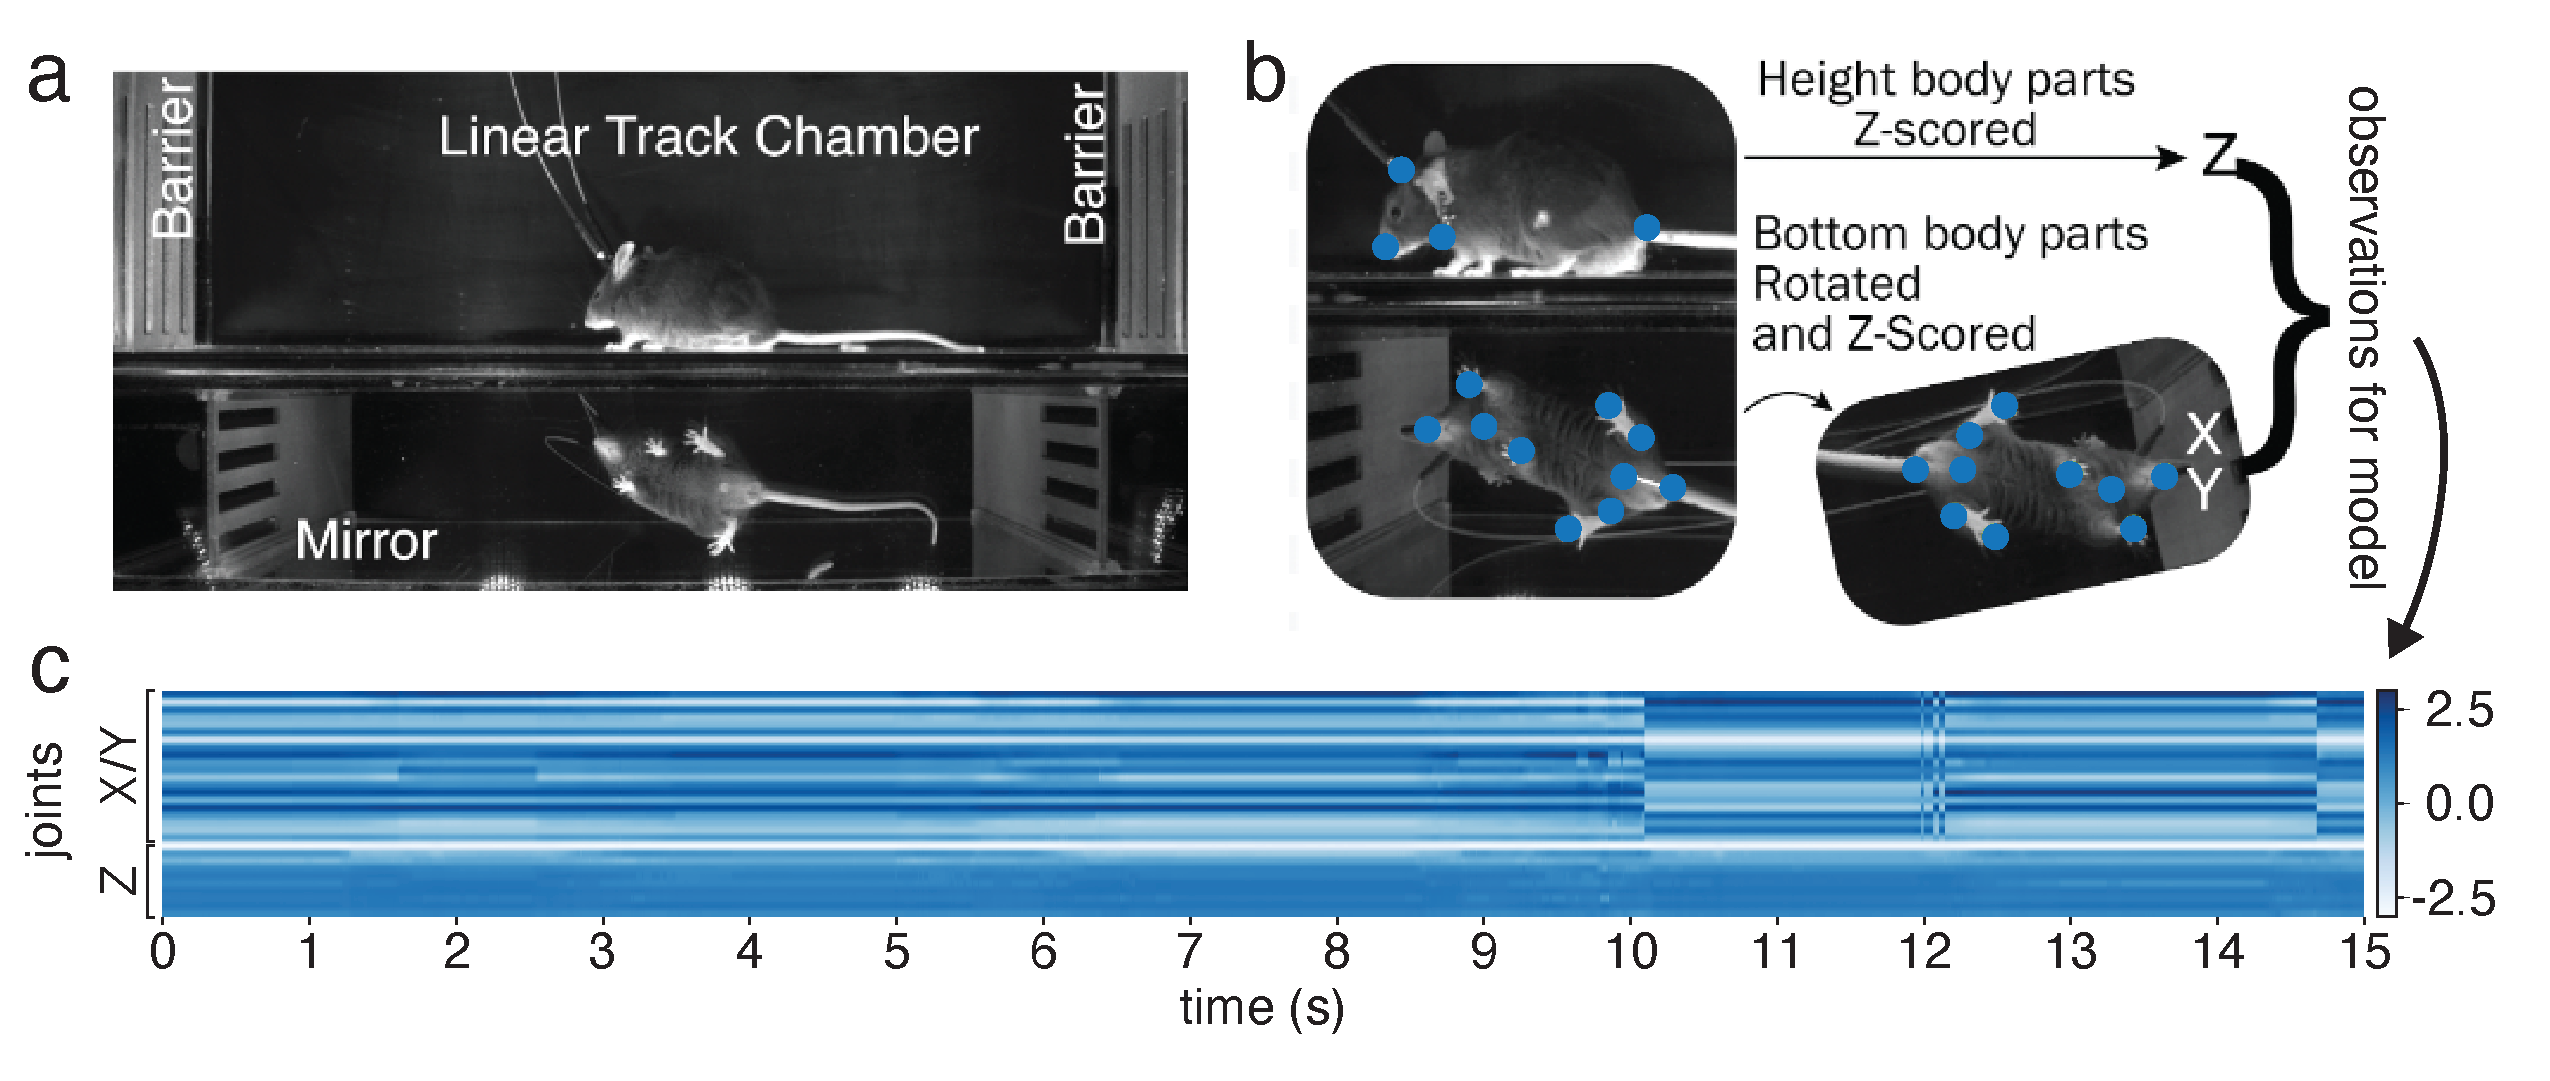
\includegraphics[width=0.90\linewidth]{ch3-slds/slds-figures/Fig1.pdf}
    \caption[Mouse body dynamics were tracked while they freely explored a linear track]{\textbf{Mouse body dynamics were tracked while they freely explored a linear track.} (a) Mice are placed into a linear track chamber with a slotted barrier on either end and a mirror underneath to provide two simultaneous views from one camera. Data are collected at 100Hz with high resolution. (b) Bottom and side body parts are tracked using SLEAP. Height information from 10 sideview body parts is z-scored. X and Y-coordinates of 10 bottomview body parts are centered, rotated, and z-scored. (c) Coordinates of side body parts (Z) is combined with bottomview coordinates (X/Y), and this combined dataset is the input to the model. }
    \label{fig:slds:1}
  \end{center}
  %\vspace{-1.5cm}
\end{figure}